\documentclass{article}
\usepackage[utf8]{inputenc}
\usepackage{amsmath, amssymb, amsthm}
\usepackage{graphicx, float}
\usepackage{hyperref}
\usepackage[dvipsnames]{xcolor}
\usepackage{algorithm}
\usepackage[noend]{algpseudocode}
\usepackage{enumitem}
\graphicspath{{../Images/}}
\usepackage{titlesec}
\titleformat{\subsection}{\LARGE\bfseries}{\thesubsection}{1em}{}


% Customization of the document
\usepackage[letterpaper, top=1.8cm, bottom=2.3cm, left=2cm, right=2cm, heightrounded]{geometry}

% Line height
\renewcommand{\baselinestretch}{1.15}

% Define the exercise counter
\newcounter{exercise}[section]   % Resets the counter every time you change the section

% Format of exercise number (e.g., 1.1-1, 1.1-2, ...)
\renewcommand{\theexercise}{\thesection.\arabic{exercise}}

% Parskip and parindent
\setlength{\parindent}{0pt}
\setlength{\parskip}{0.8em}

\title{Exercise of Getting Started}
\author{Grabur}
\date{Feb 2025}

\begin{document}

\maketitle

\section{Chapter 1: Foundations}

\subsection{The Role of Algorithms in Computing}
I didn't make the exercise of this section because I didn't find them useful.

\subsection{Getting Started}
\setcounter{exercise}{0} % Start from 0 for the exercises in this section

% Used to make a label for referencing later if it's necesary
\refstepcounter{exercise}
\textbf{Exercise 1.2-1)}:\\
It could be an application like booking. When you search a hotel close to the airport, 
it gets involved algorithms as searching the hotels close to that airport and it should be
searched in a short time period.

\refstepcounter{exercise}
\textbf{Exercise 1.2-2)}:\\
\begin{flalign*}
    8n^2 < 64n \cdot \log_2 n \quad \rightarrow \quad n < 8 \cdot \log_2 n
\end{flalign*}
Try values until this inequality is false. To $n \lessapprox 43$, insertion sort runs 
faster than merge sort.

\refstepcounter{exercise}
\textbf{Exercise 1.2-3)}:\\
\begin{flalign*}
    100n^2 < 2^n \quad 
\end{flalign*}
Trying values, for $n \lessapprox 15$, $2^n$ runs faster than $100n^2$.

\refstepcounter{exercise}
\textbf{Exercise 1.2-4)}:\\
\\
\textit{\large View photo of the exercise on the next page.}
\newpage
\begin{figure*}[h]
    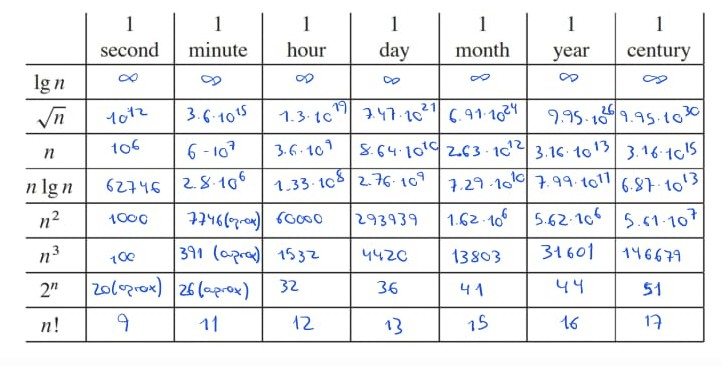
\includegraphics[scale=0.5]{Problem1_1}
    \centering
\end{figure*}


\refstepcounter{exercise}
\textbf{Exercise 2.1-1)}:\\
Note: Resolved using the logic of C, C++, Java, etc. while iterating over an array on a for
loop. Also the number that appears in \textcolor{ForestGreen}{green}, is the number being 
checked. The number or numbers that appears in \textcolor{Red}{red} are the numbers being 
moved.

\begin{center}
    \begin{tabular}{|c|c|}
    \hline
    \textbf{i} & \textbf{Array} \\
    \hline
    1) & [31, \textcolor{ForestGreen}{41}, 59, 26, 41, 58]\\
    2) & [31, 41, \textcolor{ForestGreen}{59}, 26, 41, 58]\\
    3) & [\textcolor{ForestGreen}{26}, \textcolor{Red}{31}, \textcolor{Red}{41}, 
          \textcolor{Red}{59}, 41, 58]\\
    4) & [26, 31, 41, \textcolor{ForestGreen}{41}, \textcolor{Red}{59}, 58]\\
    5) & [26, 31, 41, 41, \textcolor{ForestGreen}{58}, \textcolor{Red}{59}]\\
    \hline
    \end{tabular}
\end{center}

\refstepcounter{exercise}
\textbf{Exercise 2.1-2)}:\\
\textbf{Initialization}: The loop start getting the first number in the array. In spite of 
that, it has initialized to 0 the variable sum where the total sum will be stored. Due to 
that, the invariant holds the first number that will be added to sum.

\textbf{Maintenance}: On each iteration, the loop will hold only the index of the number 
that will be added, after add it, i will be incremented by 1, holding the next number (i + 1).

\textbf{Termination}: The loop will terminate when the 'n' elements of the array are added. In conclusion,
sum it's equivalent of say that $sum = \sum_{i = 1}^{n} A[i]$.
    
\refstepcounter{exercise}
\textbf{Exercise 2.1-3)}:\\
click this link to see the resolution \(\rightarrow \href{https://github.com/Graburr/Algorithms_CLRS_4ed_solutions/blob/main/chapter1/Getting_Started/2.1-3.cpp}
{\textcolor{blue}{resolution}}\)

\refstepcounter{exercise}
\textbf{Exercise 2.1-4)}:\\
\begin{algorithm}
\caption{Linear Search}\label{linearSearchID}
\begin{algorithmic}[1]
\Function{Linear-Search}{$A, n, x$}
    \For{$i \gets 1$ \textbf{to} $n$}
        \If {$ A[i] == x $} 
            \Return $i$
        \EndIf
    \EndFor
    \State \Return \textit{NIL}
\EndFunction
\end{algorithmic}
\end{algorithm}

\textbf{Initialization}: The loop start getting the first element of the array. 

\textbf{Maintenance}: On each iteration, the loop takes the next element (i + 1) and compare 
it with the value being search (x). If it's found return i, else, continue searching that 
value.

\textbf{Termination}: When all values are read, if x wasn't found in the array, it returns
NIL to indicate that no value was found on all the array.

\refstepcounter{exercise}
\textbf{Exercise 2.1-5)}:\\
\begin{algorithm}
\caption{ADD-BINARY-INTEGERS}\label{AddBinarySearchID}
\begin{algorithmic}[1]
\Function{ADD-BINARY-INTEGERS}{$A, B, n$}
    \State \textit{//Initialize array C with n values}
    \State \textit{carry} $\gets 0$ 
    \For {$i \gets 1$ \textbf{to} $n$}
        \State $c \gets A[i] + B[i]$
        \State $C[i] \gets c \mod 2$
        \State $carry \gets c \div 2$ \quad \textit{//Integer division}
    \EndFor
    \Statex
    \State $C[n] \gets carry$
    \State \Return \textit{C} \quad \textit{//Return the array C with the values}
\EndFunction
\end{algorithmic}
\end{algorithm}

\textbf{Initialization}: The loop starts with value of carry to 0, and getting the first 
bits of A and B.

\textbf{Maintenance}: On each iteration, the loop takes the next bits values of A and B.
Add these values and calculate the value to insert into C and the carry that could exists.

\textbf{Termination}: All values were added and store, now C[0:n - 1] with the result of 
the sum. To reach the n-th value, adds the last carry value on the position n.

\refstepcounter{exercise}
\textbf{Exercise 2.2-1)}:\\
Like the book says, \(\Theta\) notation is like saying "roughly proportional to \(n^2\) (for example), 
when \(n\) is large." In this case, we remove constants, so the remaining expression is 
\(n^3 + n^2 + n + 3\). The term with the highest exponent is \(n^3\), so at any moment:
\(n^3 \gg n^2 \gg n\). \\ 
\textbf{Solution}: \(\Theta(n^3)\).

\refstepcounter{exercise}
\textbf{Exercise 2.2-2)}:\\
\begin{algorithm}
\caption{SELECTION-SORT}\label{SelectionSortID}
\begin{algorithmic}[1]
\Function{SELECTION-SORT}{$A, n$}
    \For{$i \gets 1$ \textbf{to} $n - 1$}
        \State $ind\_small\_elm \gets i$
        \For{$j \gets i + 1$ \textbf{to} $n$}
            \If{$A[ind\_small\_elm] > A[j]$}
                \State $ind\_small\_elm \gets j$
            \EndIf
        \EndFor
        \State \Call{swap}{$A[i], A[ind\_small\_elm]$}
    \EndFor
\EndFunction
\end{algorithmic}
\end{algorithm}

The invairant is that on each iteration of extern for, it only takes 1 by 1 element. In the
inner for, also take all elemnts from i to n, and compare the value of the outter for
against the inner for to take the smaller elemnt.

When the algorithm arrives to the last element, all swaps ocurred and the last element will
be in the correct place.

The worst case happens when it must iterate on the outher for and also with al the elements
from i to n in the inner for. So it's: \(\frac{n*(n - 1)}{2}\). Thats mean that avoiding all
constants values, the solution is: \(\Theta(n^2)\).

The best case is not better because you have to check all values in the if, the only instruction
that is avoided is the instruction inside the if because the if won't be evaluated to true.
But that instruction is insignificant if \(n\) it's too big.

\refstepcounter{exercise}
\textbf{Exercise 2.2-3)}:\\
Depends on the value where is storage, if the \(x\) value is storage at the first position it
will take a constant value to search it. However, if the value is in the last element 
(worst case) it will spend \(constant * n\) time to find that value.

Averege case is suposing that it's in the middle of the array. The averegage is \(\frac{n}{2} = n\)
if \(n\) it's too big. 

Worst case as mentioned before is \(\Theta(n)\).

\refstepcounter{exercise}
\textbf{Exercise 2.2-3)}:\\
The only thing you could do is a preprocessing step to check if it's alredy sorted or nearly
to be sorted and then apply the algorithm who best fits when the best case was achieved.

\refstepcounter{exercise}
\textbf{Exercise 2.3-1)}:\\
\begin{figure*}[h]
    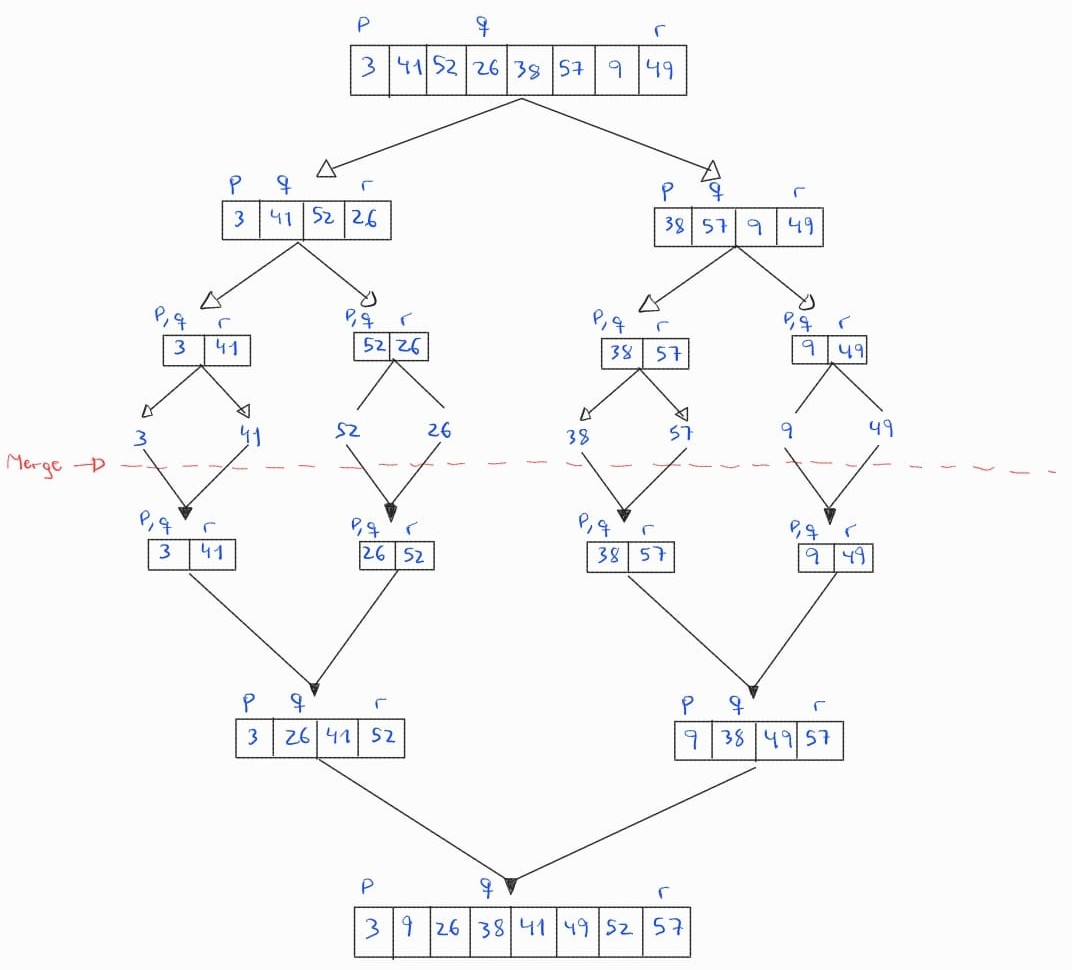
\includegraphics[scale=0.4]{Problem2_3_1.jpeg}
    \centering
\end{figure*}
\newpage

\refstepcounter{exercise}
\textbf{Exercise 2.3-2)}:\\
The "\textit{\textbf{if} \(p \neq r\)}" is not useful because \(p = 1\) and \(q > 1\), so the if
will be evaluated to true, and the return (the termination of recursion) will execute without
doing any recursion step.

\refstepcounter{exercise}
\textbf{Exercise 2.3-3)}:\\
\textbf{Initialization}: The loop starts obtaning the first element to insert it in the 
sorted array.

\textbf{Maintenance}: On each iteration, the loop insert 1 element of the left or right array,
then increment \textit{k} by 1, to insert on the next iteration the next value 1 by 1. The values
that will be inserted with the first loop in the best case is \textit{n - 1} where n is the
lenght of the subarray/array being sorted.

\textbf{Termination}: In one of the last 2 whiles, it will be inserted all remaining values
(could be values in the left or right array) until reach the nth values in the sorted array.

\refstepcounter{exercise}
\textbf{Exercise 2.3-4)}:\\
\textit{n = 2}
\[
T(2) = 2
\]
The solution given says that:
\[
T(2) = 2 * \log_2 2 = 2 \cdot 1 = 2
\]
Induction hypotesis:
\[
T(k) = k \cdot \log_2 k
\]
Where k is a power of 2. We want to demostrate that \textit{n = 2k}.
Use recurrence to calculate \(T(2k)\):
\[
T(2k) = 2T(k) + 2k \quad \rightarrow \quad T(2k) = 2 \cdot (k * \log_2 k) + 2k \quad \rightarrow
\quad T(2k) = 2k \cdot (\log_2 k + 1) \quad \rightarrow \quad T(2k) = 2k \cdot \log_2 2k
\]
As we mentiones before, replacing \textit{n = 2k}, we conclude that the induction hypotesis
is correct \textbf{\(n \cdot \log_2 n\)}

\refstepcounter{exercise}
\textbf{Exercise 2.3-5)}:\\
\begin{algorithm}
    \caption{INSERTION-SORT-RECURSIVE}\label{InsertionSortRecursiveID}
    \begin{algorithmic}[1]
        \Function{INSERTION-SORT-RECURSIVE}{$A, n$}
            \If{\(n == 0\)}  
                \Return
            \EndIf
            \State \Call{INSERTION-SORT-RECURSIVE}{$A, n - 1$}
            \State \textit{key} $\gets$ \textit{A[n]}
            \State $i \gets n - 1$
            \While {$i \geq 0$ \textbf{and} $A[i] > key$}
                \State $A[i + 1] \gets A[i]$
                \State $i \gets i - 1$
            \EndWhile
            \State $A[i + 1] \gets key$
        \EndFunction
    \end{algorithmic}
\end{algorithm}

\newpage
\refstepcounter{exercise}
\textbf{Exercise 2.3-6)}:\\
\begin{algorithm}
    \caption{BINARY-SEARCH}\label{BinarySearchID}
    \begin{algorithmic}[1]
        \Function{BinarySearch}{$A, x, l, n$}
            \If {\(l > n\)}
                \Return
            \EndIf
            \State \textit{mid} \(\gets\) \(l + n / 2\)
            \If {\(A[mid] > x\)}
                \State \Call{BinarySearch}{$A, x, l, mid - 1$}
            \ElsIf {\(A[mid] < x\)}
                \State \Call{BinarySearch}{$A, x, mid + 1, r$}
            \Else 
                \quad \Return \textit{mid}
            \EndIf
        \EndFunction
    \end{algorithmic}
\end{algorithm}

\refstepcounter{exercise}
\textbf{Exercise 2.3-7)}:\\
You can't use binary search because while you are sorting most part of the time, it won't
be that value in the sorted array. Maybe you should make a variation of binary search to 
find out in which direction has less difference betwen the number being search and then
you should move all values 1 position to right and insert in the new position.

On worst case, imagine that the worst value is at the least position, you should move
n items to the right + n / 2 that cost to search all the. So it's  \(n \cdot \frac{n}{2} = \Theta(n^2)\)

\refstepcounter{exercise}
\textbf{Exercise 2.3-8)}:
\begin{algorithm}
    \caption{FIND-SUM-TWO-ELEMENTS}\label{FindSumTwoElementsID}
    \begin{algorithmic}[1]
        \Function{FindSumTwoElements}{$S, n, x$}
            \State \Call{MergeSort}{S, 0, n - 1} \quad \textit{//\(\Theta(n * log n)\)}
            \State \( i \gets 0 \)
            \State \( j \gets n - 1 \)
            \While {\( i < j \)} \quad \textit{//\(\Theta(n)\)}
                \If {\( S[i] + S[j] = x \)}
                    \State \Return \( i, j \)
                \ElsIf {\( S[i] + S[j] < x \)}
                    \State \( i \gets i + 1 \)
                \Else
                    \State \( j \gets j - 1 \)
                \EndIf
            \EndWhile
            \State \Return \textit{No pair found}
        \EndFunction
    \end{algorithmic}
\end{algorithm}

\underline{\large{Problems of page 45}}\\
\\
\refstepcounter{exercise}
\textbf{Exercise 2-1)}:\\
\textbf{a)} The number of arrays to be sort are \(\frac{n}{k}\), where \textit{n} is the
number of elements in the original array and \textit{k} the number of elements to be sorted on
\textit{insertion sort}. Due to that, on the worst case it should be sorted \(\frac{n}{k}
\cdot k^2 \quad \rightarrow n \cdot k = \Theta(n \cdot k)\).

\textbf{b)} The recursion will be called until reach \(\frac{n}{k}\) elements on a subarray.
Hence it won't be called recursively until \(\log_2 n\) (when only 1 element is left). 
Due to that the number of recursions are delimited by \(\log_2 \frac{n}{k}\). Finally in the
worst case when only is left the first 2 subarrays, it will take \textit{n} iterations to
sort it. Due to that, we explain why it's true the expresion \(\Theta(n \cdot \log_2 \frac{n}{k})\).

\textbf{c)}  
\[
\Theta\left(n \cdot k + n \cdot \log_2 \frac{n}{k}\right) = \Theta(n \cdot \log_2 n)
\]
\[
\Theta(n \cdot k) = \Theta(n \cdot \log_2 n) \quad \rightarrow \quad k = \Theta(\log_2 n)
\]
\[
\Theta\left(n \cdot \log_2 \frac{n}{k}\right) = \Theta(n \cdot \log_2 n) \quad 
\text{//Substituting } k = \Theta(\log_2 n)
\]
\[
\Theta\left(n \cdot \log_2 \frac{n}{\log_2 n}\right) = \Theta(n \cdot \log_2 n) - \Theta(n \cdot \log_2 \log_2 n)
\quad \text{//Dominant term is  \(\Theta(n \cdot \log_2 n)\)}
\]
In conclusion, the biggest posible value which both variants of Merge Sort have the same result
is for \(k = \Theta(\log_2 n)\).

\textbf{d)}
You should see in which value it's better use one algorithm or another to sort and combine
the 2 algorithms. As we saw in the section c, this k value is calculated applying that formula.

\refstepcounter{exercise}
\textbf{Exercise 2-2)}:\\
\textbf{a)} Do you need to prove that on each iteration, of the inner for 1 element is being
moved and it remains on all iterations. In addition to that, you must prove that on the extern
for loop it's being incremented by 1.

\textbf{b) Initialization}: The loop starts taking the most right element on the array.
So the invariant is that take 1 element at a time.

\textbf{Maintenance}: Loop takes on each iteration an element, compare with the left hand
elemnt and if it's smaller than the left hand element, swap both elements. The loop invariant
remains as Initialization because on each iteration only 1 element is being checked with
another one. After that check, on the next iteration is taken the next left element.

\textbf{Termination}: When this for ends, there are a number of elements equals to \textit{i} 
(extern for) that are sorted in the lowest positions of the array.

\textbf{c)} As I said before, on each time that the inner for loop ends, 1 value is sorted.
Hence when the extern for loop ends, all values will be sorted on the right position and it's
proved the inequality.

\textbf{d)} Both have the same worst-case running time (\(\Theta(n^2)\)). But Insertion
Sort is usually better on the averegage cases because it does less swaps and usually spends
\(\Theta(n)\) on sort an array. On the other hand, Bubble Sort always spend \(Theta(n^2)\)
to sort the array. 

\refstepcounter{exercise}
\textbf{Exercise 2-3)}:\\
\textbf{a)} \(\Theta(n)\) because it has to take all values of the array \textit{A} and 
add it to \(x \cdot p\).

\textbf{b)}
\begin{figure*}[h]
    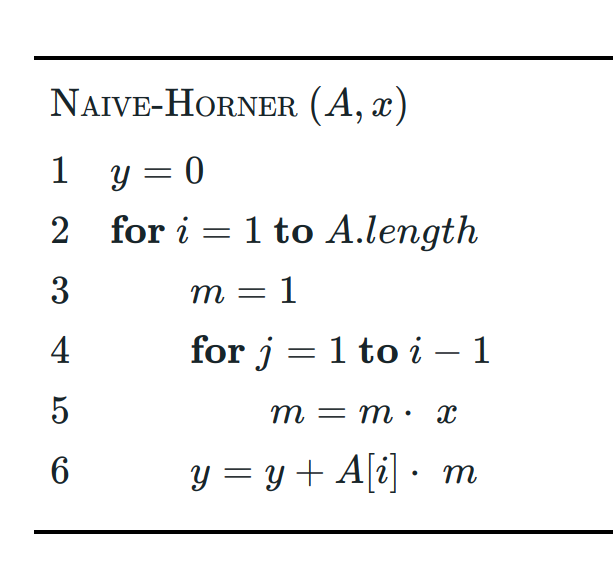
\includegraphics[scale=0.3]{Problem2_3_b}
    \centering
    \caption{Resolution extracted from \href{https://atekihcan.github.io/CLRS/02/P02-03/}
    {https://atekihcan.github.io/CLRS/02/P02-03/} I was lazy of do that hehehe.}
\end{figure*}

\textbf{c)}
For \underline{Maintenance}:
\[
y = a_i + x \sum_{k=0}^{n-(i+1)} a_{k+i+1} x^k
\]

\[
= a_i x^0 + \sum_{k=0}^{n-i-1} a_{k+i+1} x^{k+1}
\]

\[
= a_i x^0 + \sum_{k=1}^{n-i} a_{k+i} x^k
\]

\[
= \sum_{k=0}^{n-i} a_{k+i} x^k.
\]

The loop \underline{terminates} at i = -1:

\[
= a_i x^0 + \sum_{k=0}^{n-i-1} a_{k+i+1} x^{k+1} = \sum_{k=0}^{n-i} a_{k+i} x^k.
\]

\refstepcounter{exercise}
\textbf{Exercise 2-4)}:\\
\textbf{a)} Inversions are: (2, 1), (3, 1), (8, 6), (8, 1), (6, 1)

\textbf{b)} if the set is sor in ascending order, it won't be 0 inversions in the set.

\textbf{c)} Both of them are \(\Theta(n^2)\) because you have to take 1 value from the most
right position and compare if it's less than the i value (left one) on the array.

\textbf{d)}
\begin{algorithm}
    \caption{INVERSIONS}\label{InversionID}
    \begin{algorithmic}[1]
        \Function{Inversions}{$A, p, r$}
            \State \textit{//On the else of the first while of Merge, add: Print(L[i], R[j])}
        \EndFunction
    \end{algorithmic}
\end{algorithm}


\subsection{Caharcerizing Running Times}
\setcounter{exercise}{0}

\refstepcounter{exercise}
\textbf{Exercise 3.1-1)}:\\
We could do the same with saying that \textit{k} is a multiple of 2. The left subarray
has the biggests numbers, and the right one have the lowest numbers. If we want to move the
biggests numbers to the right subarray, we should move \textit{n / 2} numbers and then another
\textit{n / 2} to the left to move the lowest one at the begginig. Finally we have that
we should move \(\frac{n}{2} \cdot \frac{n}{2} = \frac{n^2}{4} = \Omega(n^2)\)

\refstepcounter{exercise}
\textbf{Exercise 3.1-2)}:\\
The extern for loop, executes in the worst case \textit{n - 1}  times. The inner loop, executes 
\textit{i + 1} to \textit{n} times. As mentioned before, the worst case is for i = 0, then
it will be executed \textit{n - 1} times. In conclusion, the wors case is \((n - 1) \cdot 
(n - 1) = O(n^2)\).

On the other hand, supose that the array is divided in 2 subarrays, the left for the higer 
values and the right for the lower ones. Althought, the extern for must iterate over all
elements, so the better case is the same as the worst (\textit{n - 1}). Then the inner loop
is the same as the worst case. The only thing that executes n/2 times is the instruction 
inside the if and the swap. These operations are constant operations. In conclusion, the
lower bound of the asymptotic behaviour is \((n - 1) \cdot (n - 1) = \Omega(n^2)\)

\textbf{\(O(n^2) = \Omega(n^2) = \Theta(n^2)\)}

\refstepcounter{exercise}
\textbf{Exercise 3.1-3)}:\\
Consideramos un array \(A\) de tamaño \(n\), dividido en tres partes:
\begin{itemize}
    \item Primera parte: Las primeras \(\alpha n\) posiciones contienen los \(\alpha n\) valores más grandes.
    \item Segunda parte: Las siguientes \((1 - 2\alpha)n\) posiciones son la parte media.
    \item Tercera parte: Las últimas \(\alpha n\) posiciones contienen los \(\alpha n\) valores más grandes después de ordenar.
\end{itemize}
El número total de movimientos es:
\[
\text{Movimientos totales} = \alpha(1 - 2\alpha)n^2.
\]
Para que el argumento tenga sentido, necesitamos que \(0 < \alpha < \frac{1}{2}\).

Maximizamos la función:
\[
f'(\alpha) = 1 - 4\alpha = 0 \quad \Rightarrow \quad \alpha = \frac{1}{4}.
\]

El número total de movimientos es:
\[
\frac{1}{4} \cdot \frac{1}{2} n^2 = \frac{1}{8}n^2.
\]
Por lo tanto, el tiempo de ejecución en el peor caso es \(\Theta(n^2)\).

\refstepcounter{exercise}
\textbf{Exercise 3.2-1)}:
\[
0 \leq c_1g(n) \leq f(n) \leq c_2g(n) = \Theta 
\]
Prove that \(\max \{f(n), g(n)\} = O(f(n) + g(n)) \quad \Rightarrow \quad \max\{f(n),g(n)\}
\leq c_2 \cdot (f(n) + g(n))\).

If the max value is \textit{f(n)}, then we have \(f(n) \leq c_2 \cdot (f(n) + g(n))\).
Also if the max value is \textit{f(n)}, then we have \(g(n) \leq c_2 \cdot (f(n) + g(n))\)
If \(c_2 = 1\), and \(n \geq n_0\), the result is \(\max \{f(n), g(n)\} = O(f(n) + g(n))\).

Prove that \(\max \{f(n), g(n)\} = \Omega(f(n) + g(n)) \quad \Rightarrow \quad \max\{f(n),
g(n)\} \geq c_1 \cdot (f(n) + g(n))\).

If the max value is \textit{f(n)}, then we have \(f(n) \geq c_1 \cdot (f(n) + g(n))\).
Also if the max value is \textit{f(n)}, then we have \(g(n) \geq c_1 \cdot (f(n) + g(n))\)
If \(c_1 = \frac{1}{2}\), and \(n \geq n_0\), the result is \(\max \{f(n), g(n)\} = \Omega
(f(n) + g(n))\).

\textbf{In conclusion}: \(\max \{f(n), g(n)\} = O(f(n) + g(n)) = \Omega(f(n) + g(n)) =
\Theta(f(n) + g(n))\) for \(c_1 = \frac{1}{2}\) and \(c_2 = 1\).

\refstepcounter{exercise}
\textbf{Exercise 3.2-2)}:\\
It's meaningless because de O notation defines asymptoticaly, the upper bound of f(n). This 
not mean \textit{"Is at least \(O(n^2)\)"} because it's only in the worst possible scenario.
Althought, we need to define the ower bound, for example the asymptotic lower bound is 
\(\Omega(n)\) that it's less than \(O(n^2)\). Hence we can't say \textit{"At least"} due to
it could spend some value betwen \(O(n^2)\) on the worst case or \(\Omega(n)\) in the best
cases.

\refstepcounter{exercise}
\textbf{Exercise 3.2-3)}:\\
With the properties of the powers, we have: 
\[
2^{n + 1} = 2^n \cdot 2^1 = O(\max\{2^n, 2^1\}) = O(2^n)
\]
The second one is wrong, because with the properties we can't remove the n there, so it
should be \(O(2^{2n})\).

\refstepcounter{exercise}
\textbf{Exercise 3.2-5)}:
\[
0 \leq c_1g(n) \leq g(n) \leq c_2g(n) = \Theta(g(n)) 
\]
\[
\Omega(g(n)) = c_1g(n) \leq g(n) \quad c_1 = \frac{1}{2} \text{ and } n \geq n_0
\]
\[
O(g(n)) = c_2g(n) \geq g(n) \quad c_2 = 2 \text{ and } n \geq n_0
\]

\refstepcounter{exercise}
\textbf{Exercise 3.2-6)}:\\
All the values of the time spent by the algorithm, will be on \(\Omega(g(n)) = g(n)
= O(g(n))\) if \(\Theta(g(n))\). Also we know that \(o(g(n)) > O(g(n))\) and 
\(\omega(g(n)) < \Omega(g(n))\), so they won't have values in common.

\refstepcounter{exercise}
\textbf{Exercise 3.2-7)}:\\
\(\Omega(g(n, m)) = \{ f(n, m)\) : if there exists a constant \textit{c}, \(n_0\) and \(m_0\) 
such that \(cg(n, m) \leq f(g, m)\) for all \( n \geq n_0\) or \(m \geq m_0\) and \(c > 0 \}\).

\(\Theta(g(n, m)) = \{ f(n, m)\) if there exists a constant \(c_1\), \(c_2\), \(n_0\) and 
\(m_0\) such that \(0 \leq < c_1g(n, m) \leq g(n, m) \leq c_2g(g, m)\) for all \(n \geq n_0\)
or \(m \geq 0\) and \(c_1 > 0\), \(c_2 > 0 \}\).

\refstepcounter{exercise}
\textbf{Exercise 3.3-1)}:\\
\textit{f(n)} is monotically increasing because there is an \(f(m) \leq f(n)\). For \textit{g(n)}
it's the same. Then we have: 
\[
f(m_1) \leq f(n_1) + g(m_2) \leq g(n_2) \quad \Rightarrow f(m_1) + g(m_2) \leq f(n_1) + g(n_2)
\]
Demostrate \(f(g(n))\):
\[
f(g(m)) \leq f(g(n)) \quad m \leq n
\]
Demostrate \(f(n) \cdot g(n)\) are non negative for an \(n_1 > 0, n_2 > 0, m_1 < n_1 and m_2 < n_2\) 
\[
f(m_1) * g(m_2) \leq f(n_1) * g(n_2)
\]

\refstepcounter{exercise}
\textbf{Exercise 3.3-2)}:
\[
\lfloor \alpha n \rfloor = \alpha n \quad \quad \lceil (1 - \alpha)n \rceil = (1 - \alpha)n
\]
\[
\alpha n + (1 - \alpha)n = n(\alpha + 1 - \alpha) = n
\]

\refstepcounter{exercise}
\textbf{Exercise 3.3-3)}:\\
Applying the properties of exponentials, we have
\[
(n + o(n))^k = n^k + o(n^k) \quad \Rightarrow \quad \Theta(\max \{n^k, n^k\}) = \Theta(n^k)
\]
With the property of ceil and floor, we know \(\lceil n \rceil^k \leq n^k \leq \lfloor n 
\rfloor^k\), the problem says \(\Theta(n^k) = n^k\)

\refstepcounter{exercise}
\textbf{Exercise 3.3-4)}:
\begin{enumerate}[label=\alph*)]
    \item Equation \(a^{\log_b c} = c^{\log_b a}\)
    \[
    \log_b c = x \quad \quad \log_b a = y
    \]
    \[
    a^x = (b^y)^x \quad \Rightarrow \quad a^{\log_b c} = b^{yx}
    \]
    Use the relation \(c = b^x\)
    \[
    c^y = (b^x)^y \quad \Rightarrow \quad c^{\log_b a} = b^{xy}
    \]
    \[
    a^{\log_b c} = b^{yx} = c^{\log_b a}
    \]
    \newpage
    \item Demostrate equations 3.26, 2.27 y 3.28.

    3.26) 
    \[
    n! = \sqrt{2\pi n} * \left(\frac{n}{e}\right)^n + 1 \quad \Rightarrow \quad (2\pi n)^
    \frac{1}{2} * \left(\frac{n}{e}\right)^n + 1
    \]
    Removing the constant values that are \(2, \pi, e, 1\), the reamining values are:
    \(n^{\frac{1}{2}} \cdot n^n = o(n^n)\).

    3.27)
    \[
    n! \approx \sqrt{2 \pi n} \left(\frac{n}{e}\right)^n.
    \]
    Prove \( n! = \omega(2^n) \), that's mean:
    \[
    \frac{n!}{2^n} \to \infty.
    \]

    Dividiendo por \( 2^n \),
    \[
    \frac{n!}{2^n} \approx \sqrt{2\pi n} \left(\frac{n}{2e}\right)^n.
    \]
    For a bigger value of \( n \) , \( \frac{n}{2e} > 1 \), the term tends to infinity.
    We can conclude that
    \[
    n! = \omega(2^n).
    \]
    \item \(\log_2(\Theta(n)) = \Theta(\log_2 n)\)
    \[
    \log_2(c_1 \cdot n) \leq \log_2(f(n)) \leq \log_2(c_2 \cdot n) \quad \Rightarrow \quad
    \log_2 c_1 + \log_2 n \leq \log_2(f(n)) \leq \log_2 c_2 + \log_2 n.
    \]
    \(\log_2 c_1\) and \(\log_2 c_2\) are constants. Hence we have: \(\log_2(f(n)) = 
    \Theta(\log_2 n) \quad \Rightarrow \quad \log_2(\Theta(n)) = \Theta(\log_2 n)\)
\end{enumerate}

\refstepcounter{exercise}
\textbf{Exercise 3.3-5)}:\\
As we saw, \(\lceil \log_2 n \rceil! = \log_2 n!\) applying the formula 3.28, we have that
\(\log_2 n = \Theta(n \log_2 n)\). In conclusión, it's polinomially bounded.

\(\lceil \log_2{\log_2 n} \rceil! = \log_2{\log_2 n} = \log_2{\Theta{n * \log_2 n}}\)
with that we can show that is \textbf{not} polinomally bounded.

\refstepcounter{exercise}
\textbf{Exercise 3.3-6)}:\\
for the definition, we know \(\log_2^* n < 5\) (rarely will be upper to 5). If we supose that
takes the value of \(n = 2^{65536} = 10^{\frac{65536}{\log_2 10}} \approx 10^{19.728}\) The result of
\(\log_2^* 10^19.728 = 5\) for example, then we have \(\log_2 5 \approx  2.322\).

On the other hand, for the same \textit{n} value, we have \(\log_2 10^19.728 \approx 65.535\)
then looking the table, Applying the logarithm iteratively, we can see:
\begin{enumerate}
    \item \(\log_2 65.535 \approx 6.02\).
    \item \(\log_2 6.02 \approx 1.37\)
    \item \(\log_2 1.37 \approx 0.45\)
\end{enumerate}
Because we could apply 3 times the iteration, \(\log_2^*(\log_2 n) = 3\).
\textbf{In conclusion}, \(\log_2^*(\log_2 n) >\) \(\log_2(\log_2^* n)\)

\refstepcounter{exercise}
\textbf{Exercise 3.3-7)}:\\
Substitute \(\phi = \frac{1 + \sqrt{5}}{2}\) in \(x^2 = x + 1\).
\[
\left(\frac{1 + \sqrt{5}}{2}\right)^2 = \frac{1 + \sqrt{5}}{2} + 1 \quad \Rightarrow \quad
\frac{3 + \sqrt{5}}{2} = \frac{3 + \sqrt{5}}{2}  
\]
With the \(\widehat{\phi}\) is do the same procedure.

\refstepcounter{exercise}
\textbf{Exercise 3.3-9)}:\\
supose \(\log_2 k = \log_2 n\), then operating we have: 
\[
\frac{k * \log_2 n}{\log_2 n} = \Theta\left(\frac{n}{\log_2 n}\right) \quad \Rightarrow \quad
k = Theta\left(\frac{n}{\log_2 n}\right)
\]

\subsection{Divide and Conquer}
\setcounter{exercise}{0}

\refstepcounter{exercise}
\textbf{Exercise 4.1-1)}:\\
\(T(n) = 8T(\lfloor\frac{n}{2}\rfloor + \Theta(1))\). As mentioned before, the ceil and floor
doesn't matter on anylizing algorithms when \textit{n} is too big. Due to that, the result
is the same \(T(n) = \Theta(n^3)\).

\refstepcounter{exercise}
\textbf{Exercise 4.1-2)}:\\
The length of the matrix that you pass as a fourth parameter, now it should be \(k * n\), for
bigger values of n and k, is the same as says, \(T(n) = 8T(\frac{k * n}{2}) + \Theta(1)\).
Now the result is \(T(n) = \Theta(k * n^3)\). 

The second option is the same as the first one. Inconclusion any of them is asymptoticaly
faster than the other one, both of them have the same speed.

\refstepcounter{exercise}
\textbf{Exercise 4.1-3)}:\\
Now is \(\Theta(n^2)\) the driving function because you need to combine the solutions.
Then \(T(n) = 8T(\frac{n}{2}) * \Theta(n^2)\). Applying the master theorem, \(n^{\log_2 8}
= 3\), case 1 applies again. \(f(n) = O(n^{3 - \epsilon})\) for any positive \(\epsilon \leq
1\)












\end{document}
